\chapter{Implementation}
\label{implementation}

\section{Integer Linear Programming}
For prototype the ILP problem formulated in the section 3.1.1 was modeled and solved in AMPL language.

\begin{lstlisting}[caption=AMPL model]

set Tier; 
set VM;

param tier_used{Tier, VM}; 
param vm_used{VM};
param cpu_demand{Tier};
param mem_demand{Tier};
param cpu_max{VM};
param mem_max{VM};
param use_tier_weight{Tier, VM};
param use_vm_weight{VM};
param not_use_tier_weight{Tier, VM};
param not_use_vm_weight{VM};

var tier_usage{Tier, VM} >= 0 binary;
var vm_usage{VM} >= 0 binary;
var tier_idle{Tier, VM} >= 0 binary;
var vm_idle{VM} >= 0 binary;
var cpu{Tier, VM} >= 0 integer;
var mem{Tier, VM} >= 0 integer; 

minimize cost:
  sum{i in Tier, j in VM} 
    (use_tier_weight[i, j] * tier_usage[i, j] +
      not_use_tier_weight[i, j] * tier_idle[i, j]) + 
  sum{j in VM} (use_vm_weight[j] * vm_usage[j] + 
    not_use_vm_weight[j] * vm_idle[j]);

subject to CPU_availability{j in VM}:
  sum{i in Tier} 
    cpu[i, j] <= cpu_max[j] * vm_usage[j];

subject to RAM_availability{j in VM}:
  sum{i in Tier} mem[i, j] <= mem_max[j];

subject to CPU_demand{i in Tier}:
  sum{j in VM} cpu[i, j] = cpu_demand[i];

subject to RAM_demand{i in Tier}:
  sum{j in VM} mem[i, j] = mem_demand[i];

subject to CPU_activation{i in Tier, j in VM}:
  cpu_max[j] * tier_usage[i, j] >= cpu[i, j];

subject to RAM_activation{i in Tier, j in VM}:
  mem_max[j] * tier_usage[i, j] >= mem[i, j];

subject to CPU_RAM_activation{i in Tier, j in VM}:
  mem_max[j] * cpu[i, j] >= mem[i, j];

subject to RAM_CPU_activation{i in Tier, j in VM}:
  cpu_max[j] * mem[i, j] >= cpu[i, j];

subject to link_tier_idle{i in Tier, j in VM}:
  tier_idle[i, j] + tier_usage[i, j] = 1;

subject to link_vm_idle{j in VM}:
  vm_idle[j] + vm_usage[j] = 1;
\end{lstlisting}

In the executor we solve the problem using \textit{or-tools} and ILP solver by Google. The Solver component
accepts the current allocation, the topology and provides as output a new allocation. The new allocation is
the input of the Translator component which translates the new allocation to the list of actions to be run.
This list of actions is the input to the Executor component.

\section{API}
\subsection{Main Node}
\textbf{[GET] /api/allocation}
Returns the allocation JSON of known VMs. In reality, just make calls to VMs and groups answers.
\begin{lstlisting}[caption=Example GET allocation output,basicstyle=\tiny]
{
  "52.34.2.170": {
    "rubis_app_server":{  
      "cpuset": [0],
      "cpu_cores": 1,
      "mem_units": 2
    },
    "pwitter_app_server":{  
      "cpuset": [1],
      "cpu_cores": 1,
      "mem_units": 3
    }
  }
}
\end{lstlisting}

\vspace{5mm}
\textbf{[GET] /api/inspect}
Returns the inspect output JSON for known VMs. In reality, just make calls to VMs and groups answers.
\begin{lstlisting}[caption=Example GET inspect output,basicstyle=\tiny]
{
  "52.34.2.170": {  
    "rubis_app_server":{  
     "MemUnits": 2,
      "CpusetCpus": "0",
      "Memory":1073741824
    },
    "pwitter_app_server": {  
      "MemUnits": 3,
      "CpusetCpus": "1",
      "Memory": 1610612736
    }
  } 
}
\end{lstlisting}

\vspace{5mm}
\noindent\textbf{[GET] /api/topology} \\
Returns JSON with the current topology.
\begin{lstlisting}[caption=Example topology,basicstyle=\tiny]
{
  "infrastructure": {
    "cloud_driver": {
      "name": "aws-ec2",
      "autoscaling_group_name": "monolithic-ex-8cpu",
      "credentials": "/usr/me/utils/aws.properties"
    },
    "max_vms": 10,
    "hooks_git_repo": "https://github.com/n43jl/hooks.git"
  },
  "apps": [{
    "name": "rubis",
    "tiers": {
      "loadbalancer": {
        "name": "Front Load Balancer",
        "max_node": 1,
        "docker_image": "haproxy",
        "depends_on": ["app_server"],
        "on_dependency_scale": "reload_server_pool.sh",
        "max_rt": 0.1
      },
      "app_server": {
        "name": "Application Logic Tier",
        "docker_image": "polimi/rubis-jboss",
        "depends_on": ["db"],
        "on_node_scale": "jboss_hook.sh",
        "on_dependency_scale": "reload_connections.sh",
        "ports": ["80:8080"],
         "entrypoint_params": "-w 3 -k eventlet"
      },
      "db": {
        "name": "Data Tier",
        "max_node": 1,
        "docker_image": "mysql",
        "on_node_scale": "mysql_hook.sh",
        "max_rt": 0.2,
        "ports": ["3306:3306"]
      }
    }
  },{
    "name": "pwitter",
    "tiers": {
      "app_server": {
        "name": "Application Logic Tier",
        "docker_image": "pwitter-web",
        "ports": ["8080:5000"],
        "entrypoint_params": " /opt/jboss-4.2.2.GA/bin/run.sh --host=0.0.0.0 
        --bootdir=/opt/rubis/rubis-cvs-2008-02-25/Servlets_Hibernate -c default"
      },
      "db": {
        "name": "Data Tier",
        "max_node": 1,
        "docker_image": "mysql",
        "on_node_scale": "mysql_hook.sh",
        "max_rt": 0.2,
        "ports": ["3307:3306"]
      }
    }
  }],
} 
\end{lstlisting}

\vspace{5mm}
\noindent\textbf{[PUT] /api/topology} \\
Set the topology. The payload is the same as the example output of the [GET] /api/topology method.

\vspace{5mm}
\noindent\textbf{[PUT] /api/translate} \\
Returns JSON with the actions list required to execute provided in the payload plan.
\begin{lstlisting}[caption=Example of the input payload,basicstyle=\tiny]
{
  "rubis": {
    "app_server": {
      "cpu_cores": 1,
      "mem_units": 3
    }
  },
  "pwitter": {
    "app_server": {
      "cpu_cores": 1,
      "mem_units": 4  
    }
  }
}
\end{lstlisting}
\begin{lstlisting}[caption=Example of the output,basicstyle=\tiny]
{  
  "actions":[  
    "update container \"rubis_app_server\" 
     on the vm "52.34.2.170" set cpu_cores=1 and mem_units=3",
    "update container \"pwitter_app_server\" 
     on the vm "52.34.2.170" set cpu_cores=1 and mem_units=4"
  ]
}
\end{lstlisting}



\subsection{Agent}
\textbf{[GET] /api/allocation} \\
Returns JSON with the current allocation of the containers on the VM. The difference with the "inspect" command is that
"inspect" is the output of "docker inspect" command, while the "allocation" is taken from the app runtime state. e.g. We
create using the API some container "Jboss". Both the "allocation" and "inspect" will return 1 container. After that we 
stop / start our Executor Agent Node. The "allocation" will be empty, but the "inspect" will return 1 container.
\begin{lstlisting}[caption=Example GET allocation output,basicstyle=\tiny]
{  
  "rubis_app_server":{  
    "cpu_cores": 1,
    "mem_units": 2
  },
  "pwitter_app_server":{
    "cpu_cores": 1,
    "mem_units": 3
  }
}
\end{lstlisting}

\vspace{5mm}
\noindent\textbf{[GET] /api/inspect} \\
Returns JSON with the current docker containers running on the VM.
\begin{lstlisting}[caption=Example GET inspect output,basicstyle=\tiny]
{  
  "rubis_app_server":{  
    "MemUnits": 2,
    "CpusetCpus": "0",
    "Memory":1073741824
  },
  "pwitter_app_server": {  
    "MemUnits": 3,
    "CpusetCpus": "1",
    "Memory": 1610612736
  }
}
\end{lstlisting}

\vspace{5mm}
\noindent\textbf{[GET] /api/topology} \\
The output is the same as for the main node.

\vspace{5mm}
\noindent\textbf{[PUT] /api/topology} \\
The input and the output is the same as for the main node.

\vspace{5mm}
\noindent\textbf{[PUT] /api/translate} \\
Returns JSON with the actions list required to execute provided in the payload plan.
\begin{lstlisting}[caption=Example of the input payload,basicstyle=\tiny]
{
  "rubis": {
    "app_server": {
      "cpu_cores": 1,
      "mem_units": 3
    }
  },
  "pwitter": {
    "app_server": {
      "cpu_cores": 1,
      "mem_units": 4  
    }
  }
}
\end{lstlisting}
\begin{lstlisting}[caption=Example of the output,basicstyle=\tiny]
{  
  "actions":[  
    "update container \"rubis_app_server\" set cpu_cores=1 and mem_units=3",
    "update container \"pwitter_app_server\" set cpu_cores=1 and mem_units=4"
  ]
}
\end{lstlisting}

\vspace{5mm}
\noindent\textbf{[PUT] /api/topology} \\
Set the topology. The payload is the same as the example output of the [GET] /api/topology method.

\vspace{5mm}
\noindent\textbf{[PUT] /api/execute} \\
Returns JSON with the actions list required to execute provided in the payload plan.
\begin{lstlisting}[caption=Example of the input payload,basicstyle=\tiny]
{
  "rubis": {
    "app_server": {
      "cpu_cores": 1,
      "mem_units": 3
    }
  },
  "pwitter": {
    "app_server": {
      "cpu_cores": 1,
      "mem_units": 4  
    }
  }
}
\end{lstlisting}

\vspace{5mm}
\noindent\textbf{[PUT] /api/run/tier\_hooks} \\
Returns JSON with the actions list required to execute provided in the payload plan.
\begin{lstlisting}[caption=Example of the input payload,basicstyle=\tiny]
[
  {
    "app": "rubis",
    "dependent": "app_server",
    "depends_on": ["db"],
    "allocation": "..."
  }
]
\end{lstlisting}

\vspace{5mm}
\noindent\textbf{[PUT] /api/docker/run} \\
Runs the docker container specified in the payload.
\begin{lstlisting}[caption=Example of the input payload,basicstyle=\tiny]
{
  "name":"pwitter_app_server",
  "cpu_cores": 2,
  "mem_units": 3
}
\end{lstlisting}

\noindent\textbf{[PUT] /api/docker/remove} \\
Removes the docker container specified in the payload.
\begin{lstlisting}[caption=Example of the input payload,basicstyle=\tiny]
{  
  "name":"pwitter_app_server"
}
\end{lstlisting}

\noindent\textbf{[PUT] /api/docker/update} \\
Returns JSON with the actions list required to execute provided in the payload plan.
\begin{lstlisting}[caption=Example of the input payload,basicstyle=\tiny]
{  
  "name":"pwitter_app_server",
  "cpu_cores": 1,
  "mem_units": 2
}
\end{lstlisting}


\section{Topology}
There are restrictions for the topology:
\begin{enumerate}
    \item Ports are specified in the form (host VM port : guest container port). All hosts ports specified for all tiers should be unique, even for different applications.
    \item The script name specified in the "on\_node\_scale" should be located in the repository specified in "hooks\_git\_repo" in the folder "scale\_hooks".
    \item The script name specified in the "on\_dependency\_scale" should be located in the repository specified in "hooks\_git\_repo" in the folder "tier\_hooks".
    \item The max\_node=1 means that the tier is not scalable. It will not be moved from one VM to another and it must have the resources demand less than it is available on one VM.
    \item For tiers with the max\_node \textgreater{} 1 is allowed to have dependencies only to tiers with max\_node=1 (n-to-1). n-to-n dependencies are not allowed.
    \item Dependencies between tiers from different applications are not allowed.
    \item Circular dependencies are not allowed
\end{enumerate}

Also tier names should be unique inside the app, and the app name should be unique too. Any tiers of any apps can be on the same VM, so uniqueness of the container name is imposed by using as container name the compound name: "{APP\_NAME}\_{TIER\_NAME}".

\section{Hooks}
To adjust to the new allocation they should be provided with input parameters.

The "on\_node\_scale" hook requires as the input parameter the previous resources and the new. So there are 4 input parameters: previous CPU cores, previous memory units, new CPU cores and new memory units.

The "on\_dependency\_scale" hook requires the IP address of the dependee tier and new allocation resources. So the input parameters are: the dependee tier name, the dependent tier name and stringified allocation JSON.

\section{Algorithms}
\subsection{Processing list of actions}
\begin{figure}[ht]
  \centering
    \includegraphics[height=550px,natwidth=219,natheight=635]{./pictures/algorithm1}
    \caption{Processing list of actions }
\end{figure}
The algorithm figure 4.1 describes the workflow in processing the list of actions for containers and processing hooks. First of all the tiers that depends on other tiers should be processed only after the dependee. To support this we build the dependency graph and process tiers without dependencies first and after remove them from the graph.

The second is the order of processing a tier. We should first create containers, after we can do update and only after that we can do remove. This is done to have more resources than it required for the tiers, otherwise the monitor component may detect that applications needs more resources.

All the hooks (scale-hooks and tier-hooks) are run only they are specified for this tier.


\subsection{Processing plan}
\begin{figure}[ht]
  \centering
    \includegraphics[height=550px,natwidth=202,natheight=714]{./pictures/algorithm2}
    \caption{Processing the plan }
\end{figure}
Processing the plan is specified in the figure 4.2.
While processing the plan, the plan "app -\textgreater{} tier -\textgreater{} demand" is flatten to the form "app\_tier -\textgreater{} demand". 
If the demand is not equal to allocation than the ILP formulation is built and solved. As the result we get the new resource allocation considering VMs and containers with resources on them.
The procedure "process list of actions" is described in the figure 4.1.

\clearpage
\subsection{Translation}

The goal of the translation is to express the new allocation as the list of actions considering the current allocation. The set of possible actions considering we the container with the name "app\_tier" and the VM with the IP "127.0.0.1":
\begin{itemize}
    \item Create VM '127.0.0.1'
    \item Delete VM '127.0.0.1'
    \item Create container 'app\_tier' on the VM '127.0.0.1' with cpu=2 and mem=2.5gb
    \item \begin{sloppypar}Update container 'app\_tier' on the VM '127.0.0.1' set cpu=1 and mem=1gb\end{sloppypar}
    \item Run scale\_hooks for the container 'app\_tier' on the VM '127.0.0.1'
    \item Delete container 'app\_tier" on the VM '127.0.0.1'
    \item Run tier\_hooks for the container 'app\_tier' on the VM '127.0.0.1'
\end{itemize}

The algorithm for this translation is:
\begin{lstlisting}[caption=Translation algorithm]
FOR ALL vm IN current_allocation:
  IF vm IN new_allocation:
    FOR ALL container IN current_allocation[vm]:
      IF not container IN new_allocation[vm]:
        push_delete_container_action
  ELSE:
    push_delete_vm_action
FOR ALL vm IN new_allocation:
  IF vm IN current_allocation:
    FOR ALL container IN new_allocation[vm]:
      IF container IN old_allocation[vm]:
        push_update_container_action_if_needed
        push_run_scale_hooks_if_needed
      ELSE:
        push_create_container_action
        push_run_scale_hooks_if_needed
  ELSE:
    push_create_vm_action
    FOR ALL container IN new_allocation[vm]:
      push_create_container_action
      push_run_scale_hooks_if_needed
\end{lstlisting}

Scale-hooks run after each container update / create. Tier-hooks can be handled only considering the dependency graph. The executor adds tier-hooks to the list of actions.

\section{Monolithic vs Hierarchical approach}

\begin{figure}[ht]
  \centering
    \includegraphics[width=350px,natwidth=684,natheight=687]{./pictures/arch-hierachical}
    \caption{Hierarchical Executor}
\end{figure}

The current approach with solving a plan using ILP formulation we call the "monolithic" approach. Considering that all the implementation is run in the MAPE framework environment for the monolithic approach we have a global planner. Having a global planner has some drawbacks, as the control loop timeout should be at least the time required to run the plan (considering the VM creation take a long time for our test it was approximately 150s).

To go around large control loop timeouts we decided that MAPE components can be hierarchically spread among all the VMs and containers. So instead of having the one global planner, we want to have planner for each container. This we call the hierarchical approach.

\section{Drivers}
There were implemented several drivers for managing virtual / cloud infrastructure: Vagrant, AWS, Docker.

As vagrant is an interface (a facade) to large list of different virtualization providers and AWS also supports very large list of vitalization (even Docker containers). This 3 cases covers a lot of different virtualization techniques.

\subsection{Vagrant driver}
Vagrant was used mostly during the implementation stage of the work to test everything locally without paying for Amazon AWS infrastructure.

The image for Vagrant is based on the "ubuntu/trusty64" image with docker and "Ecoware executor agent" installed.

All ports that are required for tiers should be preconfigured in the Vagrantfile. The application "Ecoware executor agent" uses the port 8000, which should be also preconfigured in the Vagrant file. The Vagrant configuration files can be found in the repository.

Vagrant is something like an interface or a facade to list of the virtualization providers. As providers Vagrant supports:
\begin{itemize}
    \item VirtualBox
    \item VMware
    \item Hyper-V
    \item Docker
    \item You can develop your own plugin for custom provider
\end{itemize}
Using Vagrant helps to abstract from different providers and make it easy to change providers without changing our driver.

To manage Vagrant our driver uses the python module \textit{subprocess} to call OS commands like \textit{vagrant up}

\subsection{AWS driver}
For implementing AWS driver it were tested 3 different ways to communicate with AWS:
\begin{enumerate}
    \item HTTP REST calls
    \item AWS management console
    \item Python AWS SDK boto3
\end{enumerate}
As all the code for the paper was written in the python, it was decided that using boto3 is the simplest and cleanest way.

In current implementation it was easier to use the AWS Auto Scaling Groups to create VMs. So creating VMs now is based on the "desired capacity" method for Auto Scaling Groups in AWS. So the workflow for creating VMs now is:
\begin{enumerate}
    \item Get required VM number from ILP solution (n).
    \item Set desired capacity for the Auto Scaling Group to n.
    \item Poll number of instances in the Auto Scaling Group until it equals to n.
    \item Poll the status of all instances of the Auto Scaling Group to be the "in service".
    \item Get IP addresses of all VMs.
    \item Analyse the previous allocation, the new allocation and separate existed machines with the new.
    \item Set the topology to the new VMs, on error sleep 10s and repeat.
\end{enumerate}

The "polling" in this context means to make the request to the AWS and if the result is not satisfactory, sleep 10s, and repeat the request again.

Creating the VM takes approximately 150s.

For the deletion of the VM we can not just set the desired capacity to the smaller number, because we need to delete some particular machine, but not any one from all machines. To remove particular machine we just do 2 actions:
\begin{enumerate} 
    \item Detach the instance from the autoscaling group.
    \item Terminate the instance
\end{enumerate}

The AWS infrastructure supports different virtualization techniques:
\begin{itemize}
    \item HVM
    \item PV
    \item Docker containers
\end{itemize}
HVM stands for Hardware-Assisted Virtualization. 
PV stands for Paravirtualization.
In spite of the fact that these virtualization techniques are different and have its own advantages and disadvantages, AWS helps us to abstract from this and use its unified API.

To configure AWS for using with AWS driver it is required to do some steps:
\begin{description}
    \item [AMI.] The AMI should contain the \textit{Ecoware Executor Agent} and docker installed. The \textit{Ecoware Executor Agent} and docker engine should be in the autostart. All the containers images that will be used for different tiers should be pulled in the docker. Also all the containers should be removed to not have the name collision.
    \item [Security Group.] Security Group should be configured considering all the ports that containers want to listen to and the \textit{Ecoware Executor Agent} default port 8000.
    \item [Launch Configuration.] Launch Configuration should be created considering the AMI we want to use, the security group, and the AWS instance type.
    \item [Auto Scaling Group.] Auto Scaling Group should be created using the Launch Configuration with the initial instance number equals to 0.
\end{description}

\subsection{Docker driver}
Besides the fact that both Vagrant and AWS support Docker containers as under layer virtualization technique (or the provider), we use docker without any facade or interface, but directly. This helps to simplify and separate the separation between fine-grained and coarse-grained virtualization.

Docker is managed as the Vagrant using OS calls with the python module \textit{subprocess}.

\begin{sloppypar}The command to run have this structure (example of the run action):\end{sloppypar}

\begin{lstlisting}[caption=Docker run template,basicstyle=\small]
docker run -itd {PORTS} {HOSTS} --cpuset-cpus={CPUS} 
  -m={MEM}m --name={NAME} -v=/ecoware:/ecoware {IMAGE} 
  {ENTRY_PARAMS}
\end{lstlisting}

\begin{lstlisting}[caption=Docker run example,basicstyle=\small]
docker run -itd -p 8080:5000 --add-host="db:172.31.31.123"
  --cpuset-cpus=0,1 -m=512m --name=rubis_app_server 
  -v=/ecoware:/ecoware pwitter-web -w 3 -k eventlet
\end{lstlisting}

\textit{-it} option means to allocate a tty for the container process (to run it interactively).\\
\textit{-d} option means to run container in the \textit{detached} mode (background mode).\\
The variable \textit{\{PORTS\}} is built considering ports specified in the topology.\\
The variable \textit{\{HOSTS\}} is built if the tier has dependency n-to-1 or 1-to-1.\\
Variables \textit{\{CPUS\}} and \textit{\{MEM\}} is resources demand from the plan.\\
The variable \textit{\{NAME\}} is built from the topology like\\ "\{APP\_NAME\}\_\{TIER\_NAME\}".\\
\textit{-v} option means to add a data volume. The format is host\_dir:guest\_dir. The name of the directory is hardcoded, this is directory where the git repository with hooks is pulled.\\
The variable \textit{\{IMAGE\}} is taken from the topology.\\
The variable \textit{\{ENTRY\_PARAMS\}} is the entry point params also taken from the topology.


\section{Unit testing}
Some of the algorithms can be easily tested with unit-testing.

For example, the ILP algorithm is quite weight sensitive and tuning the weights can break some logic. Moreover there are many different ways how the system can satisfy the new plan and sometimes it is not clear and obvious which way is more optimal. So for the ILP solver it was written a list of the tests.

The input for the test is 3 json files: "plan.json", "result.json" and "allocation.json". So the iLP solver is tested that given the current allocation and the plan, it produces the new allocation equals to specified in the "result.json".

Any arguable ILP solution can be inspected in details and added to the tests.

Also algorithms like "building the dependency graph", "translation from allocation to actions" are tested too.

\section{UML}
\begin{figure}[ht]
  \centering
    \includegraphics[width=350px,natwidth=633,natheight=482]{./pictures/implementation-main}
    \caption{Class diagram for the executor on the Main Node}
\end{figure}

\begin{figure}[ht]
  \centering
    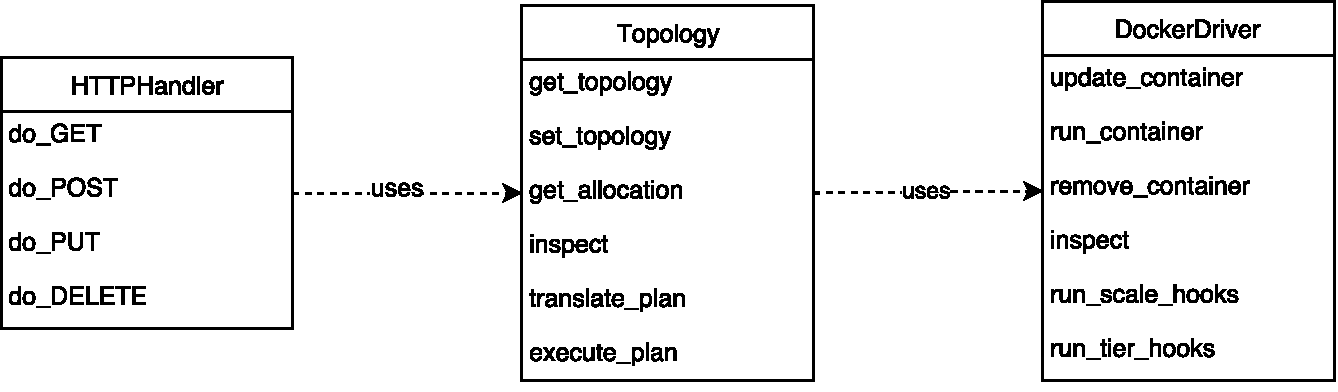
\includegraphics[width=350px,natwidth=643,natheight=190]{./pictures/implementation-agent}
    \caption{Class diagram for the executor on the Agent Node}
\end{figure}

\begin{figure}[ht]
  \centering
    \includegraphics[height=450px,natwidth=433,natheight=593]{./pictures/sequence}
    \caption{Sequence diagram}
\end{figure}
